\documentclass[a4paper,14pt]{extarticle}

\usepackage[utf8x]{inputenc}
\usepackage[T1,T2A]{fontenc}
\usepackage[russian]{babel}
\usepackage{hyperref}
\usepackage{indentfirst}
\usepackage{here}
\usepackage{array}
\usepackage{graphicx}
\usepackage{caption}
\usepackage{subcaption}
\usepackage{chngcntr}
\usepackage{amsmath}
\usepackage{amssymb}
\usepackage{pgfplots}
\usepackage{pgfplotstable}
\usepackage[left=2cm,right=2cm,top=2cm,bottom=2cm,bindingoffset=0cm]{geometry}
\usepackage{multicol}

\renewcommand{\le}{\ensuremath{\leqslant}}
\renewcommand{\leq}{\ensuremath{\leqslant}}
\renewcommand{\ge}{\ensuremath{\geqslant}}
\renewcommand{\geq}{\ensuremath{\geqslant}}
\renewcommand{\epsilon}{\ensuremath{\varepsilon}}
\renewcommand{\phi}{\ensuremath{\varphi}}

\counterwithin{figure}{section}
\counterwithin{equation}{section}
\counterwithin{table}{section}
\newcommand{\sign}[1][5cm]{\makebox[#1]{\hrulefill}} % Поля подписи и даты
\graphicspath{{pics/}} % Путь до папки с картинками
\captionsetup{justification=centering,margin=1cm}
\def\arraystretch{1.3}


\begin{document}

\begin{titlepage}	% начало титульной страницы

	\begin{center}		% выравнивание по центру

		\large Санкт-Петербургский Политехнический Университет Петра Великого\\
		\large Институт компьютерных наук и технологий \\
		\large Кафедра компьютерных систем и программных технологий\\[6cm]
		% название института, затем отступ 6см
		
		\huge Метрология, стандартизация и сертификация\\[0.5cm] % название работы, затем отступ 0,5см
		\large Отчет по лабораторной работе №2\\[0.1cm]
		\large <<Регулятор мощности>>\\[6cm]

	\end{center}


	\begin{flushright} % выравнивание по правому краю
		\begin{minipage}{0.30\textwidth} % врезка в половину ширины текста
			\begin{flushleft} % выровнять её содержимое по левому краю

				\large\textbf{Работу выполнил:}\\
				\large Ламтев А.Ю.\\
				\large {Группа:} 23501/4\\
				
				\large \textbf{Преподаватель:}\\
				\large Кошелев С.И.

			\end{flushleft}
		\end{minipage}
	\end{flushright}
	
	\vfill % заполнить всё доступное ниже пространство

	\begin{center}
	\large Санкт-Петербург\\
	\large \the\year % вывести дату
	\end{center} % закончить выравнивание по центру

\thispagestyle{empty} % не нумеровать страницу
\end{titlepage} % конец титульной страницы

\vfill % заполнить всё доступное ниже пространство


\tableofcontents
\newpage

\section{Моделирование схемы в OrCAD Capture}

\subsection{Исходная схема}

На рисунке \ref{pic:scheme} изображена схема регулятора мощности. (файл \textbf{Регулятор\_мощности.doc})

\begin{figure}[H]
\begin{center}
	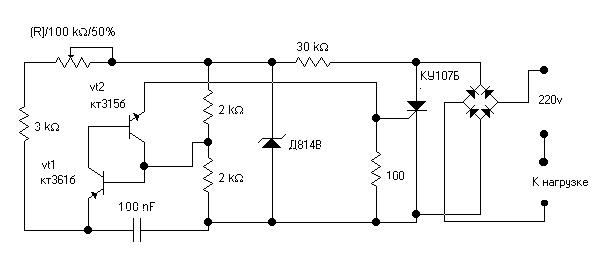
\includegraphics[width=1\textwidth]{scheme}
	\caption{Схема регулятора мощности}
	\label{pic:scheme}
\end{center}
\end{figure}

Данная схема используется в регуляторах яркости люстры и регуляторах температуры паяльника.

На вход схемы подается напряжение $220$ В $50$ Гц. Затем через диодный мост КЦ405А ток идет на параметрический стабилизатор, образованный резистором $30$ кОм и стабилитроном Д814В. Стабилитрон Д814В служит для стабилизации и ограничения возможного повышения напряжения, питающего схему управления, а резистор $30$ кОм гасит лишнее напряжение и напряжение опускается до напряжения стабилитрона Д814В. Дальше напряжение поступает на переменный резистор $100$ кОм и резистор $2$ кОм. Переменный резистор соединяется резистором $3$ кОм и конденсатором $100$ нФ с транзистором КТ361Б. На этой цепочке образуется задержка сигнала периодов тока, который подается на эмиттер КТ361Б. Как только на нём напряжение становится больше чем напряжение в точке соединения резисторов $2$ кОм и $2$ кОм, транзисторы открываются и весь накопленный на конденсаторе 100 нФ ток поступает на управляющий электрод тиристора, открывая его. Затем напряжение через диодный мост идет на нагрузку. Изменением сопротивления переменного резистора регулируется скорость разрядки конденсатора, от которой зависит напряжение, поступающее на нагрузку.

Свойством, оценка которого позволит судить о качестве работы устройства, выбрано - \textbf{диапозон регулируемой мощности}.

\subsection{Элементы схемы}

В таблице \ref{tab:transistors} представлены основные параметры транзисторов \verb+КТ315Б+, \verb+BC846+, \verb+КТ361Б+ и \verb+Q2N4250+. Транзисторы \verb+КТ315Б+ и \verb+КТ361Б+ являются элементами исходной схемы, а \verb+BC846+ и \verb+Q2N4250+ соответственно их аналогами, которые есть в библиотеке \textbf{PSpice} и будут использованы при моделировании.

\begin{table}[H]
\begin{center}
	\caption{Основные параметры транзисторов}
	\label{tab:transistors}
	\def\tabcolsep{10pt}
	\begin{tabular}{|l|l|l|l|l|l|l|}
		\hline
		Наименование &
		тип & 
		$I_k$, А &
		$U_\text{кэ}$, В & 
		$P$, Вт & 
		$F$, МГц & 
		$\beta_{min}$ \\ 
		\hline
		КТ315Б &
		n-p-n &
		0.1 &
		20 &
		0.15 &
		250 &
		50 \\
		\hline
		BC846 &
		n-p-n &
		0.1 &
		65 &
		0.33 &
		250 &
		110 \\
		\hline
		КТ361Б &
		p-n-p &
		0.05 &
		20 &
		0.15 &
		250 &
		50 \\
		\hline
		Q2N4250 &
		p-n-p  &
		0.05 &
		25 &
		&
		500 &
		500 \\ 
		\hline
\end{tabular}
\end{center}
\end{table}

В таблице \ref{tab:diods} представлены основные параметры диодов \verb+КЦ405А+ и \verb+MUR160+. Диод \verb+КЦ405А+ является элементом исходной схемы, а \verb+MUR160+ - это его аналог, который есть в библиотеке \textbf{PSpice} и будет использован при моделировании.

\begin{table}[H]
\begin{center}
	\caption{Основные параметры диодов}
	\label{tab:diods}
	\def\tabcolsep{10pt}
	\begin{tabular}{|l|l|l|l|}
		\hline
		Наименование &
		$I_\text{пр max}$, А &
		$U_\text{обр}$, В &
		$U_\text{пр}$, В \\ 
		\hline
		КЦ405А &
		1 &
		600 &
		4 \\
		\hline
		MUR160 &
		1 &
		600 &
		1.35 \\
		\hline
\end{tabular}
\end{center}
\end{table}

В таблице \ref{tab:stabilitrons} представлены основные параметры стабилитронов \verb+Д814В+ (который используется в исходной схеме) и \verb+D1N758+ (аналог, который есть в библиотеке \textbf{PSpice} и будет использован при моделировании).

\begin{table}[H]
\begin{center}
	\caption{Основные параметры стабилитронов}
	\label{tab:stabilitrons}
	\def\tabcolsep{10pt}
	\begin{tabular}{|l|l|l|l|l|}
		\hline
		Наименование &
		$U_\text{ст}$, В &
		$I_\text{ст}$, мА &
		$I_\text{ст max}$, мА &
		$R_\text{дифф}$, Ом \\ 
		\hline
		Д814В &
		9---10.5 &
		3 &
		32 &
		12 \\
		\hline
		D1N758 &
		10 &
		20 &
		35 &
		17 \\
		\hline
\end{tabular}
\end{center}
\end{table}

В таблице \ref{tab:thyristors} представлены основные параметры тиристоров \verb+КУ208Г+ (который используется в исходной схеме) и \verb+MAC228A6+ (аналог, который есть в библиотеке \textbf{PSpice} и будет использован при моделировании).

\begin{table}[H]
\begin{center}
	\caption{Основные параметры тиристоров}
	\label{tab:thyristors}
	\def\tabcolsep{4pt}
	\begin{tabular}{|c|c|c|c|c|c|c|c|}
		\hline
		Наименование &
		$I_\text{пр ос}$, А &
		$U_\text{пр}$, В &
		$U_\text{вкл}$, В &
		$I_\text{зс}$, мА &
		$U_\text{отп}$, В &
		$t_\text{вкл}$, $\mu$с &
		$t_\text{выкл}$, $\mu$с \\ 
		\hline
		КУ208Г &
		5 &
		2 &
		400 &
		5 &
		5 &
		10 &
		150 \\
		\hline
		MAC228A6 &
		8 &
		2 &
		400 &
		5 &
		10 &
		1.5 &
		\\
		\hline
		%MCR729-6 &
		%5 &
		%1.5 &
		%400 &
		%10 &
		%5 &
		%0.4 &
		%15 \\
		%\hline
\end{tabular}
\end{center}
\end{table}

В таблице \ref{tab:elements_analogs} представлено соответствие элементов исходной схемы и их аналогов.

\begin{table}[H]
\begin{center}
	\caption{Активные элементы исходной схемы и их аналоги}
	\label{tab:elements_analogs}
	\def\tabcolsep{10pt}
	\begin{tabular}{|l|l|l|}
		\hline
		Класс элемента &
		Элемент исходной схемы & 
		Аналог \\
		\hline
		Транзистор &
		КТ315Б &
		BC846 \\
		\hline
		Транзистор &
		КТ361Б &
		Q2N4250 \\
		\hline
		Диод &
		КЦ405А &
		MUR160 \\
		\hline
		Стабилитрон &
		Д814В &
		D1N758 \\
		\hline
		Тиристор &
		КУ208Г &
		MAC228A6 \\
		\hline
\end{tabular}
\end{center}
\end{table}

\subsection{Схема моделирования}

Для построения схемы моделирования, изображённой на рис. \ref{pic:mod_scheme}, была создана библиотека содержащая \textbf{PSpice} модели элементов схемы, УГО которых приведено  в соответствие с ЕСКД. 

В процессе моделирования процесса регулировки мощности устройства на вход подавалось сетевое напряжение $220$ В $50$ Гц, и на нагрузке (резистор $R7$) снимались напряжение и мощность в течение $20$ миллисекунд (полный период синусоиды). Это производилось для разных значений резистора $R4$ в диапозоне $0\dots100$ кОм

\begin{figure}[H]
\begin{center}
	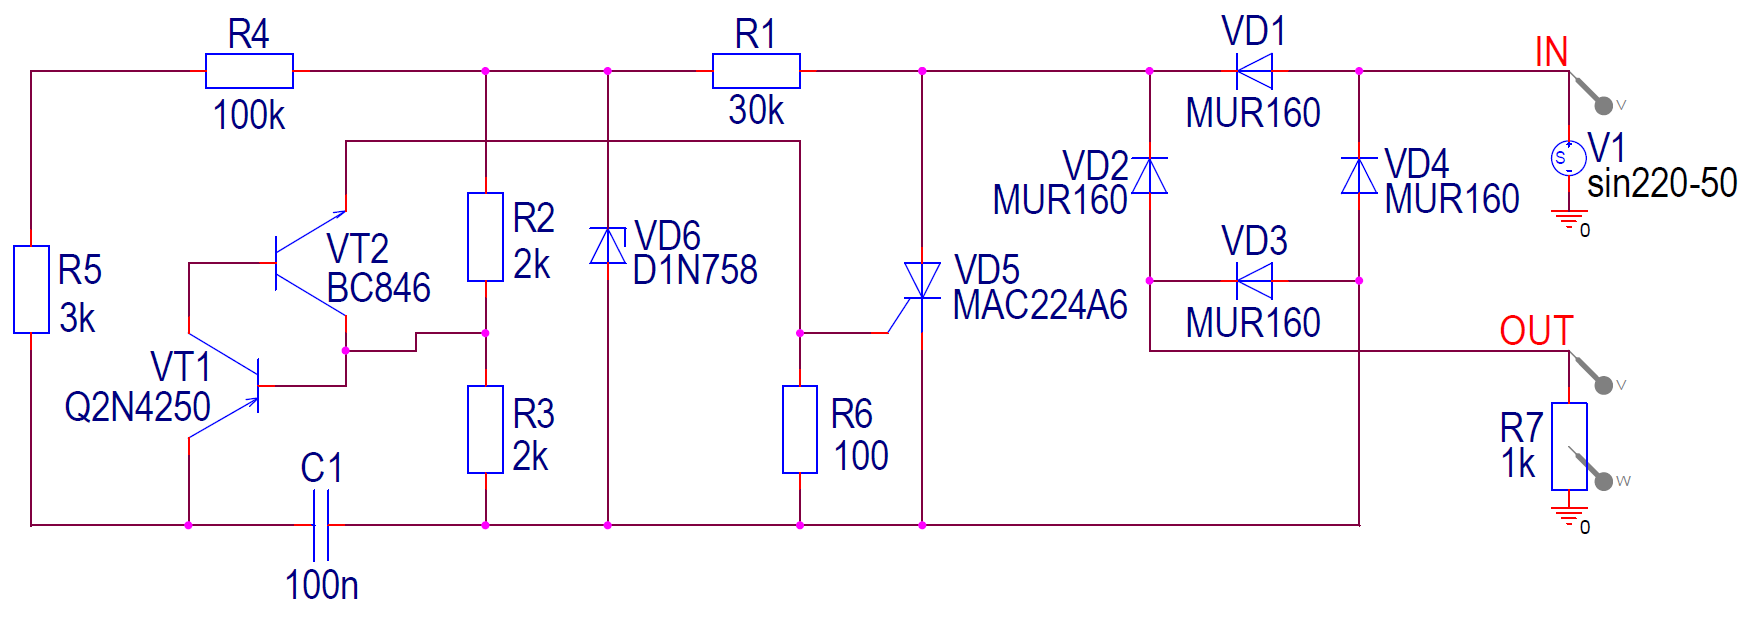
\includegraphics[width=1\textwidth]{modeling_schema}
	\caption{Схема моделирования}
	\label{pic:mod_scheme}
\end{center}
\end{figure}

\subsection{Результаты моделирования}

В результате моделирования процесса регулировки мощности устройства были построены временые диаграммы.

\subsection{Измеряемые величины}

\section{Оценка априорной инструментальной погрешности измерений}

\subsection{Методы измерений}

\subsection{Средства измерений}

\subsection{Погрешность измерений}

\end{document}
